% Authors: David Padilla Orenga, Ignacio Pastore Benaim
\documentclass{article}
\usepackage[utf8]{inputenc}
\usepackage[linesnumbered,ruled,vlined]{algorithm2e} 
\usepackage[a4paper, margin=1in, top=0.25in, bottom=1in, left=0.75in, right=0.75in]{geometry}
\title{Assignment 3 \\ \small Introduction to Parallel Programming.}
\author{David Padilla Orenga\\ Ignacio Pastore Benaim}
\date{}  

\usepackage{graphicx}
\usepackage{amsmath}
\usepackage{hyperref}
\usepackage{color}

% Hyphen penalty
\hyphenpenalty=10000
\exhyphenpenalty=10000
\sloppy

\begin{document}

\maketitle

\section*{Virtual Machine Specifications}
The laboratory was executed in a Virtual Machine (VM) with the following specifications:

\begin{table}[h!]
\centering
\begin{tabular}{|l|l|}
\hline
\textbf{Specification} & \textbf{Details} \\ \hline
Architecture           & ARM64 (aarch64)  \\ \hline
Machine Type           & QEMU 7.2 ARM Virtual Machine \\ \hline
Memory                 & 4 GB             \\ \hline
Disk Size              & 21.38 GB         \\ \hline
\end{tabular}
\end{table}

\section*{Question 1: Mutual Exclusion for Correctness}
Yes, mutual exclusion is critical for ensuring the correctness of multithreaded programs. In the absence of mutual exclusion mechanisms, shared resources accessed by multiple threads simultaneously can lead to race conditions. Race conditions occur when the behavior of a program depends on the relative timing of thread execution, often producing unpredictable results.

\textbf{Role of \texttt{std::mutex}:}  
A \texttt{std::mutex} ensures that only one thread at a time can access a critical section of code or a shared resource. For example, consider a producer-consumer problem where both producer and consumer threads access a shared buffer. Without a \texttt{std::mutex}, multiple threads might modify the buffer simultaneously, leading to data corruption.

\textbf{Example:}  
\begin{verbatim}
std::mutex mtx;
void critical_section() {
    std::lock_guard<std::mutex> lock(mtx);
    // Critical code here
}
\end{verbatim}

\textbf{Role of \texttt{std::condition\_variable}:}  
While \texttt{std::mutex} prevents race conditions, \texttt{std::condition\_variable} ensures efficient coordination between threads. For instance, a consumer thread can wait for a signal from the producer thread, avoiding busy-waiting and conserving CPU cycles.

\textbf{Key Benefits:}  
The combination of \texttt{std::mutex} and \texttt{std::condition\_variable} allows for safe, efficient interaction between threads, ensuring correctness and optimal resource usage.

\section*{Question 2: Thread Pool Destructor}
Proper implementation of the thread pool destructor is essential to ensure that all resources are cleaned up correctly and that no tasks are left incomplete. The thread pool must ensure that:
\begin{itemize}
    \item Threads are signaled to stop execution gracefully.
    \item Tasks in the queue are processed before shutdown.
    \item All threads are joined, ensuring their complete termination.
\end{itemize}

\textbf{Steps for a Graceful Destructor:}  
1. Signal threads to stop using a flag (e.g., \texttt{done}).  
2. Notify all waiting threads using \texttt{std::condition\_variable}.  
3. Join all threads to ensure they have completed execution.

\textbf{Code Implementation:}  
\begin{verbatim}
~thread_pool() {
    done = true;
    condition_variable.notify_all();
    for (auto& t : threads) {
        if (t.joinable()) t.join();
    }
}
\end{verbatim}

\textbf{Why This Matters:}  
Without proper synchronization, threads might access resources that have already been deallocated, leading to undefined behavior. The destructor ensures that tasks are either completed or safely discarded, maintaining consistency.

\textbf{Advanced Considerations:}  
- Implementing a task queue that supports prioritized shutdowns.  
- Logging unfinished tasks for post-mortem analysis.

\section*{Question 3: Performance Analysis}
The \texttt{smallpt\_thread\_pool} binary was evaluated using different parallelization strategies. The strategies included partitioning work into rows, columns, and tiles of various sizes, such as \(128 \times 128\), \(256 \times 256\), \(16 \times 16\), and \(4 \times 4\). The goal was to assess the impact of task size on execution time and overall performance.

\subsection*{Performance Results}
Figure~\ref{fig:performance_plot} illustrates the execution times for these configurations. Smaller tiles increased parallelism but introduced significant overhead due to frequent task scheduling, while larger tiles reduced overhead but limited concurrency.

\begin{figure}[h]
    \centering
    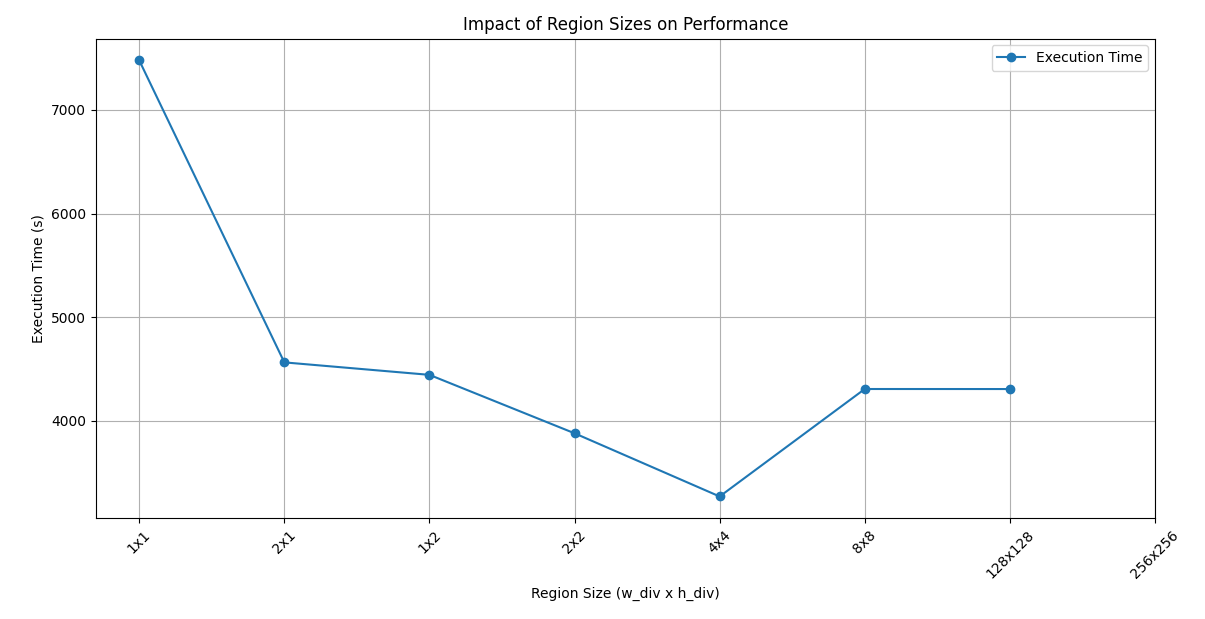
\includegraphics[width=0.8\textwidth]{./results/performance.png}
    \caption{Execution times for different parallelization strategies and region sizes.}
    \label{fig:performance_plot}
\end{figure}

\subsection*{Discussion of Results}
\begin{itemize}
    \item \textbf{Small Tiles (\(16 \times 16\)):}  
    While small tiles offer higher parallelism by creating numerous independent tasks, the overhead of task management outweighs the benefits. This results in suboptimal performance.
    \item \textbf{Large Tiles (\(256 \times 256\)):}  
    Larger tiles reduce the number of tasks, lowering overhead. However, this strategy limits parallelism, as fewer tasks are available to distribute among threads.
    \item \textbf{Medium Tiles (\(128 \times 128\)):}  
    This configuration achieved the best performance by striking a balance between task granularity and management overhead. The tile size was well-suited to the workload, dividing it into manageable chunks without overwhelming the task queue.
\end{itemize}

\subsection*{Conclusion}\vspace{-0.5em}
\noindent Based on the analysis, the \(128 \times 128\) tile size emerged as the optimal choice, offering a good balance of parallelism and efficiency. The observed errors with larger tiles underscore the importance of carefully selecting region sizes compatible with the application's requirements. Future work could explore dynamic adjustments to tile sizes based on runtime performance metrics.
\vspace{-0.5em}

\end{document}